% Options for packages loaded elsewhere
\PassOptionsToPackage{unicode}{hyperref}
\PassOptionsToPackage{hyphens}{url}
\PassOptionsToPackage{dvipsnames,svgnames,x11names}{xcolor}
%
\documentclass[
]{report}

\usepackage{amsmath,amssymb}
\usepackage{iftex}
\ifPDFTeX
  \usepackage[T1]{fontenc}
  \usepackage[utf8]{inputenc}
  \usepackage{textcomp} % provide euro and other symbols
\else % if luatex or xetex
  \usepackage{unicode-math}
  \defaultfontfeatures{Scale=MatchLowercase}
  \defaultfontfeatures[\rmfamily]{Ligatures=TeX,Scale=1}
\fi
\usepackage{lmodern}
\ifPDFTeX\else  
    % xetex/luatex font selection
\fi
% Use upquote if available, for straight quotes in verbatim environments
\IfFileExists{upquote.sty}{\usepackage{upquote}}{}
\IfFileExists{microtype.sty}{% use microtype if available
  \usepackage[]{microtype}
  \UseMicrotypeSet[protrusion]{basicmath} % disable protrusion for tt fonts
}{}
\makeatletter
\@ifundefined{KOMAClassName}{% if non-KOMA class
  \IfFileExists{parskip.sty}{%
    \usepackage{parskip}
  }{% else
    \setlength{\parindent}{0pt}
    \setlength{\parskip}{6pt plus 2pt minus 1pt}}
}{% if KOMA class
  \KOMAoptions{parskip=half}}
\makeatother
\usepackage{xcolor}
\usepackage[lmargin=30mm,rmargin=30mm]{geometry}
\setlength{\emergencystretch}{3em} % prevent overfull lines
\setcounter{secnumdepth}{-\maxdimen} % remove section numbering
% Make \paragraph and \subparagraph free-standing
\ifx\paragraph\undefined\else
  \let\oldparagraph\paragraph
  \renewcommand{\paragraph}[1]{\oldparagraph{#1}\mbox{}}
\fi
\ifx\subparagraph\undefined\else
  \let\oldsubparagraph\subparagraph
  \renewcommand{\subparagraph}[1]{\oldsubparagraph{#1}\mbox{}}
\fi


\providecommand{\tightlist}{%
  \setlength{\itemsep}{0pt}\setlength{\parskip}{0pt}}\usepackage{longtable,booktabs,array}
\usepackage{calc} % for calculating minipage widths
% Correct order of tables after \paragraph or \subparagraph
\usepackage{etoolbox}
\makeatletter
\patchcmd\longtable{\par}{\if@noskipsec\mbox{}\fi\par}{}{}
\makeatother
% Allow footnotes in longtable head/foot
\IfFileExists{footnotehyper.sty}{\usepackage{footnotehyper}}{\usepackage{footnote}}
\makesavenoteenv{longtable}
\usepackage{graphicx}
\makeatletter
\def\maxwidth{\ifdim\Gin@nat@width>\linewidth\linewidth\else\Gin@nat@width\fi}
\def\maxheight{\ifdim\Gin@nat@height>\textheight\textheight\else\Gin@nat@height\fi}
\makeatother
% Scale images if necessary, so that they will not overflow the page
% margins by default, and it is still possible to overwrite the defaults
% using explicit options in \includegraphics[width, height, ...]{}
\setkeys{Gin}{width=\maxwidth,height=\maxheight,keepaspectratio}
% Set default figure placement to htbp
\makeatletter
\def\fps@figure{htbp}
\makeatother
% definitions for citeproc citations
\NewDocumentCommand\citeproctext{}{}
\NewDocumentCommand\citeproc{mm}{%
  \begingroup\def\citeproctext{#2}\cite{#1}\endgroup}
\makeatletter
 % allow citations to break across lines
 \let\@cite@ofmt\@firstofone
 % avoid brackets around text for \cite:
 \def\@biblabel#1{}
 \def\@cite#1#2{{#1\if@tempswa , #2\fi}}
\makeatother
\newlength{\cslhangindent}
\setlength{\cslhangindent}{1.5em}
\newlength{\csllabelwidth}
\setlength{\csllabelwidth}{3em}
\newenvironment{CSLReferences}[2] % #1 hanging-indent, #2 entry-spacing
 {\begin{list}{}{%
  \setlength{\itemindent}{0pt}
  \setlength{\leftmargin}{0pt}
  \setlength{\parsep}{0pt}
  % turn on hanging indent if param 1 is 1
  \ifodd #1
   \setlength{\leftmargin}{\cslhangindent}
   \setlength{\itemindent}{-1\cslhangindent}
  \fi
  % set entry spacing
  \setlength{\itemsep}{#2\baselineskip}}}
 {\end{list}}
\usepackage{calc}
\newcommand{\CSLBlock}[1]{\hfill\break\parbox[t]{\linewidth}{\strut\ignorespaces#1\strut}}
\newcommand{\CSLLeftMargin}[1]{\parbox[t]{\csllabelwidth}{\strut#1\strut}}
\newcommand{\CSLRightInline}[1]{\parbox[t]{\linewidth - \csllabelwidth}{\strut#1\strut}}
\newcommand{\CSLIndent}[1]{\hspace{\cslhangindent}#1}

\usepackage[noblocks]{authblk}
\renewcommand*{\Authsep}{, }
\renewcommand*{\Authand}{, }
\renewcommand*{\Authands}{, }
\renewcommand\Affilfont{\small}
\makeatletter
\@ifpackageloaded{caption}{}{\usepackage{caption}}
\AtBeginDocument{%
\ifdefined\contentsname
  \renewcommand*\contentsname{Table of contents}
\else
  \newcommand\contentsname{Table of contents}
\fi
\ifdefined\listfigurename
  \renewcommand*\listfigurename{List of Figures}
\else
  \newcommand\listfigurename{List of Figures}
\fi
\ifdefined\listtablename
  \renewcommand*\listtablename{List of Tables}
\else
  \newcommand\listtablename{List of Tables}
\fi
\ifdefined\figurename
  \renewcommand*\figurename{Figure}
\else
  \newcommand\figurename{Figure}
\fi
\ifdefined\tablename
  \renewcommand*\tablename{Table}
\else
  \newcommand\tablename{Table}
\fi
}
\@ifpackageloaded{float}{}{\usepackage{float}}
\floatstyle{ruled}
\@ifundefined{c@chapter}{\newfloat{codelisting}{h}{lop}}{\newfloat{codelisting}{h}{lop}[chapter]}
\floatname{codelisting}{Listing}
\newcommand*\listoflistings{\listof{codelisting}{List of Listings}}
\makeatother
\makeatletter
\makeatother
\makeatletter
\@ifpackageloaded{caption}{}{\usepackage{caption}}
\@ifpackageloaded{subcaption}{}{\usepackage{subcaption}}
\makeatother
\ifLuaTeX
\usepackage[bidi=basic]{babel}
\else
\usepackage[bidi=default]{babel}
\fi
\babelprovide[main,import]{british}
% get rid of language-specific shorthands (see #6817):
\let\LanguageShortHands\languageshorthands
\def\languageshorthands#1{}
\ifLuaTeX
  \usepackage{selnolig}  % disable illegal ligatures
\fi
\usepackage{bookmark}

\IfFileExists{xurl.sty}{\usepackage{xurl}}{} % add URL line breaks if available
\urlstyle{same} % disable monospaced font for URLs
\hypersetup{
  pdftitle={Effect of the Nominal Value of Foreign Currencies in valuing a good},
  pdfauthor={Konrad Kopp},
  pdflang={en-GB},
  pdfkeywords={Behavioural Economics, Face Value Effect, Consumer Choice
Theory},
  colorlinks=true,
  linkcolor={blue},
  filecolor={Maroon},
  citecolor={Blue},
  urlcolor={Blue},
  pdfcreator={LaTeX via pandoc}}

\title{Effect of the Nominal Value of Foreign Currencies in valuing a
good}


  \author{Konrad Kopp}
            \affil{%
                  University of Oxford
              }
      
\date{2024-04-16}
\begin{document}
\maketitle
\begin{abstract}
Research into the effect of using foreign currencies on consumption
behaviour suggests that consumers systematically under- or overspend
based on the nominal (face) value of the foreign currency. However,
previous research is undecided on which direction this effect has, with
the two most prominent models leading to different and mutually
exclusive outcomes. This paper considers the different models and tests
their predictive and explanatory accuracy using a study. It finds that
individuals tend to underspend when the foreign currency is less
numerous than (a fraction of) the home currency and overspend when the
opposite is the case.
\end{abstract}

\renewcommand*\contentsname{Table of contents}
{
\hypersetup{linkcolor=}
\setcounter{tocdepth}{2}
\tableofcontents
}
\chapter{Introduction}\label{introduction}

Past experience suggests that we treat foreign currencies differently to
our home currency and have difficulty adjusting to them. Previous
research, such as the ``money illusion'' effect suggests that
individuals are biased towards the nominal (or face value) of prices.
Past research has investigated whether a systemic effect

RAS (Raghubir and Srivastava 2002) examined the effect of using foreign
currencies on consumption behaviour and argue that there is a systematic
difference in spending behaviour based on the exchange rate of the
foreign currency to an individuals' home currency. Specifically, they
showed that when a foreign currency is a fraction of the home currency
(e.g.~1 unit in home currency is 0.2 units in foreign currency)
consumers tend to overspend in real terms relative to their home
currency. On the other hand, when the foreign currency is a multiple of
the home currency (e.g.~1 unit in home currency is 5 units in foreign
currency) consumers tend to underspend in real terms.\footnote{For
  consistency, I will use the terms fraction and multiple currencies
  throughout this paper as defined here.} RAS argue that this effect
arises because individuals are anchored on the face value of the foreign
currency which influences the exchange rate calculations from and to
their home currencies. Hence, RAS term the result of this inadequate
adjustment the face value effect.

WER (Wertenbroch, Soman, and Chattopadhyay 2007) consider the findings
by RAS and reiterate their conclusion that individuals inadequately
calculate the values of goods between differnet currencies, leading to
systematic differences in spending behaviour based on the exchange rate
between the foreign and home currencies. However, WER argue that the
process of adjustment occurs differently, namely that individuals
calculate their valuations of goods based on salient reference points,
such as budget constraints. Contrary to standard theory, WER argue that
consumers care about the difference between a valuation and their budget
rather than the ratio of the two. In the context of foreign currencies,
the nominal value of this difference will diverge, leading to systematic
differences in spending behaviour. However, the direction of this bias
is the exact opposite of the one shown by RAS. Specifically, WER show
that consumers underspend when the foreign currency is a fraction of the
home currency and overspend in the opposite case.

Fang (Fang 2019) further builds on top of the research by RAS and aims
to extend it to the domain of ``virtual'' currencies, which refers to
non-fiat currencies that are digital in nature and not controlled and
issued by a central bank. Examples of virtual currencies include video
game (or in-game) currencies, rewards points, airmiles, cryptocurrencies
and more to the extent that these are at least somewhat liquid.
Investigating in-game currencies specifically, Fang shows that consumer
valuations systematically deviate when using these currencies relative
to the home currency. Fang's findings correspond with those of RAS and
the face value effect.

This paper aims to build on the aforementioned research in several
important ways. Foremost, previous research is conclusive that there is
an effect that using foreign currencies has on individuals' consumption
behaviour relative to using their home currencies, but is divided on the
direction of this effect. Hence, this paper attempts to evaluate the
different models posed and use a study to test which model most
adequately predicts the perceived behaviour. Second, previous research
has only assigned minor significance to using incentive-compatible
mechanisms to elicit true preferences of participants. These mechanisms
have been established to elicit more accurate responses from
participants that are closer to their true preferences (\textbf{cite?}).
Hence, this study will use the Becker-DeGroot-Marshak (BDM) mechanism to
elicit participants' willingness to pay (WTP).{[}\^{} The BDM mechanism
will be defined and explained in more detail in the Methodology section
below.{]} RAS (Raghubir and Srivastava 2002) expressed the concern that
``despite attempts to make the tasks as realistic as possible, the
studies reported were laboratory experiments, and issues of
generalizability when real money is on the line do arise. For instance,
when people actually exchange foreign currency they may feel richer or
poorer depending on the exchange rate, and the differences in
perceptions of wealth may affect product valuation''. Similarly, Fang
(Fang 2019) noted that implementing the BDM mechanism was infeasible for
the study he conducted but that future research should focus on using
something like it to elicit WTP. Finally, this paper aims to extend the
previous literature on the effects of using virtual currencies
specifically, due to their increasing rise in importance when
transacting or making purchasing decisions online.

First, I present the theoretical frameworks that have been outlined by
previous research in a way that makes it easy to compare and contrast
them. These frameworks are the standard model described in consumer
choice theory, the model suggested by RAS and the model suggested by
WER. Then, I consider what each of these frameworks would predict in a
concrete case and show that all three models come to different and
mutually exclusive conclusions. In order to test which of these
frameworks is most accurate in predicting observed behaviour, I conduct
a study in which two groups each formulate their WTP for a specific good
in an incentive compatible way, with the only difference between the
groups being the exchange rate of the currency used to their home
currency and, as a result, the face values of their budget and bid.
Analysing the study, I find that consumers tend to underspend when the
foreign currency is a fraction and overspend when the foreign currency
is a multiple, which is predicted by the module proposed by WER.
However, due to the limited sample size of the study, this result is not
statistically significant and does not have significant power. Finally,
in the discussion, I will evaluate the implications of the findings for
the theoretical frameworks outlined, consider alternative explanations
for the perceived effect and argue that the model proposed by WER is the
most accurate in predicting and describing consumer behaviour when using
foreign currencies.

\chapter{Theoretical Framework}\label{theoretical-framework}

\section{Standard Model}\label{standard-model}

Standard consumer choice theory suggests that individuals formulate
valuations of goods in relation to reference points, such as their
budget (\textbf{cite?}). Specifically, standard theory poses that
consumers evaluate their valuation for a good as a ratio with the budget
in order to determine what proportion of their spending power is
required to purchase the good. To formaulate valuations of goods in a
different currency, consumers would first determine the value of the
good in their home currency and subsequently apply the exchange rate to
get their valuation in the foreign currency. Hence, the model follows a
two step process:

\begin{enumerate}
\def\labelenumi{\arabic{enumi}.}
\tightlist
\item
  Formaulate valuation of good as ratio to budget in home currency
\item
  Convert the valuation into foreign currency
\end{enumerate}

Alternatively, this can be stated using the following syntax:

\[V_n = f(\dfrac{x}{M_n})\] \[V = V_n * X = V_r\]

where V is the valuation in the foreign currency, \(V_n\) is the
valuation of the good in the home currency (nominal), \(V_r\) is the
valuation of the good in the foreign currency, \(M_n\) is the budget in
the home currency, X is the exchange rate and \(f(x)\) is some function
that uses a valuation relative to the budget in order to compute
\(V_n\).

One assumption that is implicit in this model is that a consumer will
always correctly adjust their valuation ratio based on the exact
exchange rate. However, this might not always be the most rational thing
to do. For example, when exchange rates fluctuate it might not be worth
the effort of a consumer to always use the most up-to-date exchange
rate, but rather to use some approximate value. Further, when an
individual needs to do these exchange rate calculations in their head,
it might not be worth the mental effort to calculate the amount in the
foreign currency perfectly, but an approximation might be fine. For
example, it would be rational to multiply an amount in home currency by
1.2 if the real exchange rate is 1.2113248 and the effort required is
significant, such as when attempting to calculate it in one's hand. By
loosening these assumptions, the standard model is able to account for
small deviations from a consumer's real valuation of a good in a foreign
currency.

\section{Face Value Effect Model}\label{face-value-effect-model}

RAS (Raghubir and Srivastava 2002) put forth a different model for how
consumers formulate their valuation of a good in a foreign currency
based on their studies conducted. Specifically, they pose that a
consumer will first formulate a valuation of a good in their home
currency, before converting that amount into the foreign currency using
the exchange rate. However, they argue that this calculation is biased
by the nominal value of the good in the home currency (in cases where a
consumer does not determine their valuation but observes a price, this
calculation would be biased by the nominal value of the good in the
foreign currency). This model may be formulated as follows:

\begin{enumerate}
\def\labelenumi{\arabic{enumi}.}
\tightlist
\item
  Formulate valuation of good in home currency
\item
  Convert the valuation into foreign currency
\item
  Adjust using the nominal value of good in home currency
\end{enumerate}

Alternatively, this can be stated using the following syntax:

\[V = α(V_n) + (1 - α)V_r\]

where V is the valuation in the foreign currency, \(V_n\) is the
valuation of the good in the home currency (nominal), \(V_r\) is the
valuation of the good in the foreign currency and α is a weighting
parameter such that \(α ∈[0,1]\). Importantly, RAS (Raghubir and
Srivastava 2002) argue that \(α > 0\) and that V is hence not equal to
\(V_r\) but is biased towards \(V_n\).

\section{Perceived Value of Money
Model}\label{perceived-value-of-money-model}

WER (Wertenbroch, Soman, and Chattopadhyay 2007) build on top of RAS,
but put forth a different model that they argue is more representative
of the behaviour of actual consumers. Specifically, they agree with the
standard model that valuations are made in relation to salient reference
points, such as a consumers' budget, and argue that the model put forth
by RAS fails to account for this. However, they disagree with the
standard model that valuations use a ratio of price to budget, but
instead argue that consumers think in terms of differences. Hence,
instead of considering what fraction of their purchasing power is
required to buy a good, consumers consider how much of their budget is
left over. However, WER argue that consumers inadequately adjust this
difference to the exchange rate and are thus biased when considering
goods in different currencies since the nominal differences between
price and budget will differ when considering different currencies. This
model can be formulated as follows:

\begin{enumerate}
\def\labelenumi{\arabic{enumi}.}
\tightlist
\item
  Formaulate valuation of good as difference to budget in home currency
\item
  Convert the valuation into foreign currency
\item
  Adjust using the difference to budget in the foreign currency
\end{enumerate}

Alternatively, this can be stated using the following syntax:

\[V = α(M_r - V_r) + (1 - α)V_r\]

where V is the valuation in the foreign currency, \(V_n\) is the
valuation of the good in the home currency (nominal), \(V_r\) is the
valuation of the good in the foreign currency, \(M_r\) is the budget in
the foreign currency (real) and α is a weighting parameter such that
\(α ∈[0,1]\). Importantly, WER (Wertenbroch, Soman, and Chattopadhyay
2007) argue that \(α > 0\) and that V is hence not equal to \(V_r\) but
is biased towards \(M_r - V_r\).

\section{Predictions}\label{predictions}

The three different models laid out above would each generate a
different prediction in the following scenario, considering fraction and
multiple exchange rates (the latter in brackets): a consumer values a
good at £25 and needs to express this valuation in BlueCoin. The
exchange rate of Pounds to BlueCoin is 1 BlueCoin = £5 (1 BlueCoin =
£0.2) and their budget is 10 (250) BlueCoin. The models above would make
the following predictions:

\begin{itemize}
\tightlist
\item
  Standard model: \(V_r = 5 (125) BlueCoin\)
\item
  Face value effect model: \(V_r > 5 (< 125) BlueCoin\)
\item
  Perceived value of money model: \(V_r < 5 (> 125) BlueCoin\)
\end{itemize}

where \(V_r\) is the valuation of the good in the foreign currency.

As a result:

\begin{itemize}
\tightlist
\item
  Standard model: \(V_rf = V_rm\)
\item
  Face value effect model: \(V_rf > V_rm\)
\item
  Perceived value of money model: \(V_rf < V_rm\)
\end{itemize}

where \(V_rf\) is the valuation of the good in the foreign currency for
the fraction group and \(V_rm\) is the valuation of the good in the
foreign currency for the multiple group.

In other words, the standard model would expect the valuations to be the
same across both exchange rates, the face value effect model would
expect the consumer to overspend when presented with the fraction
exchange rate and the perceived value of money model would expect the
consumer to underspend when presented with the fraction exchange rate.

\chapter{Method}\label{method}

There were 41 participants of the study, most of them current
undergraduate students at the University of Oxford, but some
participants were also recent graduates and postgraduate students. The
study took place online, using Qualtrics, and students were incentivised
to participate by taking part in a lottery, which will be explained in
further detail below.

\section{Study}\label{study}

The study itself was split into four parts: Consent Form, Introduction,
Auction and Follow-Up Questions. The entire experiment instructions can
be found in the Experiment Instructions section of the Appendix. The
first section asked participants to read through and sign the consent
form in order to ensure that they were informed about the study and what
data would be collected. In the introductory section, the BDM mechanism
was explained to participants and they were asked to complete four
question that tested their understanding of the mechanism. The aim of
this section was to ensure that participants properly understood how the
mechanism worked in order to elicit their real WTP during the main part
of the study.

The auction was the main part of the study, with the aim of eliciting
the participants' WTP on a specific item and comparing these across
different currencies used. In this section, participants were randomly
split into two groups with almost-identical instructions. The
participants were instructed to bid on the item shown below, a tabletop
airhockey table, using the virtual currency ``BlueCoin''. The auction
was explained to follow the BDM mechanism and it was also stated that
three participants of the experiment would be randomly selected, their
auction would be simulated and they would receive the outcome. The only
difference between the groups was the exchange rate between BlueCoin and
the British Pound (£) and the endowment that the participants received
in BlueCoin. The first group received an endowment of 10 BlueCoin where
1 BlueCoin equals £5 and the second group received an endowment of 250
BlueCoin where 1 BlueCoin equals £0.2. To complete the auction,
participants were asked to respond with their bid, in BlueCoin.

The final part of the experiment consisted of optional follow-up
questions that were used to determine if there are any trends in bidding
behaviour based on some characteristics of the participants. The
questions asked were about whether they had previously lived in a
different country than the UK, how often they tend to travel outside of
the UK and what their typical expenditure is in a given month. The
intention behind the first two questions is to use them as a proxy for
experience dealing with foreign currencies, where presumably people that
travel frequently or have lived in multiple countries are more
experienced with currency conversion calculations. The final question
was asked to be able to determine whether there were any systematic
differences in WTP based on a participants normal expenditure.

\section{Auction Design}\label{auction-design}

Since the aim of the study was to determine whether there were any
systematic differences in WTP between consumers when the only differing
factor is the currency used, we decided to not include a control group
that bid on the item using Pounds, which was the design of some of the
experiments run by RAS (Raghubir and Srivastava 2002). This allowed for
a simpler design and more power given the same sample size. Further,
unlike the studies run by RAS (Raghubir and Srivastava 2002) and WER
(Wertenbroch, Soman, and Chattopadhyay 2007), we did not use a fiat
currency or mix of fiat and fictional currencies, but used only one
fictional currency for both groups. On the one hand, this simplification
was due to a focus of wether the effects described in previous papers
also held in similar ways for virtual currencies. On the other hand, it
also allowed us to preclude any biases or previous experience that
participants might have had towards or with certain currencies. RAS
(Raghubir and Srivastava 2002) acknowledge that ``the face value effect
is due to the accessibility and perceptual salience of the face value of
the foreign currency \ldots{} {[}which{]} is likely to depend on the
extent to which an individual has the opportunity or the time available
to process exchange rate information and/or has experience in using a
particular foreign currency''. To bias participants the least, we chose
the relatively nondescript name for a fictional, virtual currency:
BlueCoin.

Another important decision in the design of the experiment was which
item to select that a majority of participants would have a non-zero
WTP. This is important since if the majority or even the entirety of
participants were to bid zero on the item, then we would only learn that
this was the participants' WTP for that good, but not whether there are
any systematic differences in the WTP when using different currencies.
Hence, we selected a tabletop airhockey table, something that few enough
people have so that they won't want another one, but enough people want
with a non-zero WTP, especially among a student population. In fact,
only six participants of the experiment stated a WTP of 0.

In designing the main part of the experiment, we chose to conduct an
auction, specifically using the BDM mechanism, in order to have an
incentive-compatible method of eliciting the participants' WTP. The
BDM's incentive compatibility in eliciting WTP is a well-established
phenomenon that is superior to using participants' stated preferences
(\textbf{cite?}). As mentioned above, the studies conducted by RAS
(Raghubir and Srivastava 2002), WER (Wertenbroch, Soman, and
Chattopadhyay 2007) (with the exception of one permutation of one of the
studies) and Fang (Fang 2019) did not implement incentive-compatible
methods of eliciting the participants' preferences, making this
experiment and important addition to these previous studies in examining
whether the effects describe still hold when a more accurate way of
eliciting WTP is used. In order to incentivise the participants even
further, we ran a lottery that paid out three randomly-chosen
participants based on their actual choices made in the auction and by
simulating the BDM mechanism using a random number generator. Due to
budget constraints, we were only able to play this lottery for three
people, but given that the sample size of the experiment was relatively
small, the potential to receive one's outcome is likely to have helped
in eliciting the participants' true WTP.

Finally, given our budget, we were able to give participants an
endowment of £50 each, which was around double of what the item costs to
buy. Assuming that the item is priced roughly around the average WTP
(which turned out to be correct), this endowment was chosen to leave
enough room for people with higher WTP to make their bid and for us to
capture this in the data. This is important for the goals of the
experiment, since if we had, for example, chosen an endowment of £20,
the majority of participants might have bid their maximum amount,
hindering our ability to meaningfully compare WTP across the two groups.
We chose relatively simple exchange rates of 5 and \(1/5\) so that the
exchange rate calculations would be relatively easy to make, allowing us
to be more confident that differences between groups were not due to the
mental effort required to do calculations but due to something else. RAS
(Raghubir and Srivastava 2002) acknowledge that ``the reliance on face
value may be a function of the ease with which the foreign money can be
converted. \ldots{} Future research should examine the asymmetric and
nonlinear nature of this effect''. Since the goal of this study is to
investigate that an effect exists that is not solely based on a high
difficulty or large mental effort required when doing specific,
difficult calculations, we aimed to make the calculations as easy as
possible in order to isolate the effect of the exchange rate and nominal
value of the foreign currency.

\section{Limitations}\label{limitations}

In setting up the experiment, we incorrectly used the BDM mechanism.
Instead of explaining it as a sealed-bid second-price auction, the
experiment instructions explained it as a sealed-bid first-price
auction. Unlike in a second-price auction, the participants of a first
price auction do not have a dominant strategy to bid their true
valuations, in fact there generally is no dominant strategy in such an
auction (\textbf{cite?}). (\textbf{todo?})

Another limitation of the study is the low sample size of 41
participants, which entails lower statistical power and thus a lower
likelihood of detecting a true positive when an effect actually exists.
I will examine this in further detail in the next section, conducting a
power analysis and estimating how big the sample size should have been
to achieve an adequate level of power.

\chapter{Results}\label{results}

There were 41 participants, 21 in the first group and 20 in the second.
To conduct the data analysis, I have normalised the bids across both
groups by converting them into pounds and computed the following summary
statistics:

\begin{verbatim}
   Min. 1st Qu.  Median    Mean 3rd Qu.    Max.    NA's 
   0.00   10.00   20.00   19.74   32.00   50.00      20 
\end{verbatim}

\begin{verbatim}
[1] 15.49001
\end{verbatim}

\begin{verbatim}
   Min. 1st Qu.  Median    Mean 3rd Qu.    Max.    NA's 
   0.00   16.50   27.50   25.57   35.25   50.00      21 
\end{verbatim}

\begin{verbatim}
[1] 14.8083
\end{verbatim}

Further, I plotted the following boxplot, in order to visually see the
difference between the groups:

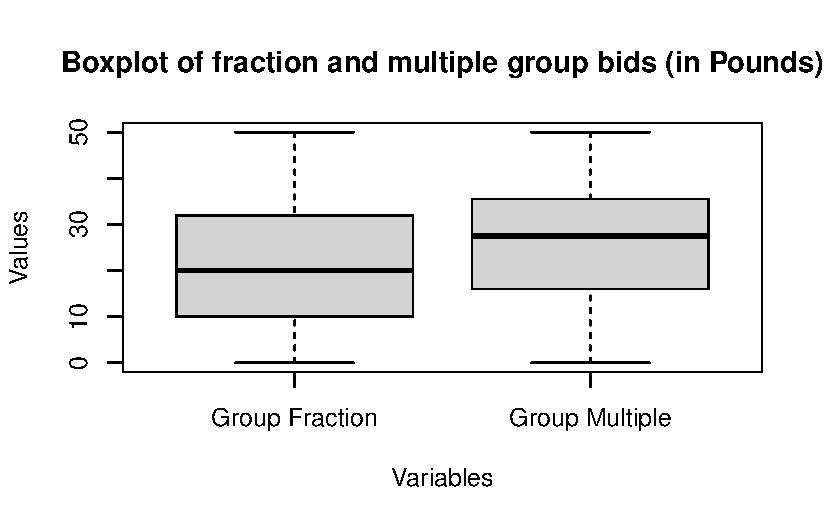
\includegraphics{paper_files/figure-pdf/unnamed-chunk-2-1.pdf}

As is obvious from the summary statistics and the boxplot, there is a
difference between both groups, namely that the bids in the multiple
group seem to be higher on average than those in the fraction group. To
investigate this hypothesis, I conducted a t-test of a difference in
means between the groups, specifically a Welch Two Sample t-test. The
null hypothesis is that the difference in means is equal to 0 (or,
alternatively, that the means are the same) and the alternative
hypothesis is that this difference is not equal to 0 (or, alternatively,
that the means are not the same):

\[h_0: µ_1 = µ_2\] \[h_1: µ_1 ≠ µ_2\]

Hence, I conducted the t-test:

\begin{verbatim}

    Welch Two Sample t-test

data:  experiment_data$group_fraction_bid_in_pounds and experiment_data$group_multiple_bid_in_pounds
t = -1.2323, df = 38.999, p-value = 0.2252
alternative hypothesis: true difference in means is not equal to 0
95 percent confidence interval:
 -15.401901   3.740092
sample estimates:
mean of x mean of y 
  19.7381   25.5690 
\end{verbatim}

The t-value of -1.2323 suggests that there is a difference in the means
between the groups and, since it is negative, that the mean of the
fraction group is lower. However, the p-value is 0.2252, which is quite
high. If we take the typical significance level of \(α = 0.05\) we find
that the p-value is higher than this value, and thus fail to reject the
null hypothesis at the 5\% significance level. Further, the 95\%
confidence interval is \([-15.401901, 3.740092]\) which includes 0,
providing further evidence that the difference in means between the
groups is not statistically significant. Thus, we must conclude that
while there seems to be a difference in means based on the sample data,
this difference is not statistically significant for this sample size.

To investigate this further, I have conducted a power analysis in order
to determine the power of the t-test, which refers to the likelihood of
the test detecting a true positive when an effect actually exists
(\textbf{cite?}). High power would indicate that this likelihood is high
and vice versa. To conduct the analysis, we first need to find the
effect size, or Cohen's D and then implement the power analysis.
Further, I will also conduct an analysis that investigates how big the
sample size should have been to get a power of 80\%.

\begin{verbatim}

     t test power calculation 

             n1 = 21
             n2 = 20
              d = 0.3845806
      sig.level = 0.05
          power = 0.2246363
    alternative = two.sided
\end{verbatim}

\begin{verbatim}

     Two-sample t test power calculation 

              n = 107.1047
              d = 0.3845806
      sig.level = 0.05
          power = 0.8
    alternative = two.sided

NOTE: n is number in *each* group
\end{verbatim}

Based on the first test with the same significance level of 0.05, we can
see that the power is 0.2246363 or 22\%, which means that there is only
a 22\% likelihood of detecting a true positive if an effect actually
exists. In other words, the likelihood of detecting a true difference in
means between the two groups, when this difference exists, is only 22\%,
which is far below the usual value of 80\%. The second test takes in
this power of 80\% and calculates the required sample size at the
observed effect size. The result is \(n = 107\) where the sample size is
\(2n\) or 214. Hence, using a sample size of 214 and observing the same
effect, this t-test would yield a power of 80\% at the 5\% significance
level.

Finally, I conducted a regression of the demographic values collected in
the fourth part of the experiment on the bids of each group. This is
done in order to determine whether there is any correlation between the
demographic variables and the bid amount, which would suggest that
randomisation did not occur correctly, which could have been exacerbated
by the small sample size. The regression yields the following outcomes:

\begin{verbatim}

Call:
lm(formula = group_fraction_bid_in_pounds ~ lived_abroad + travel_frequency + 
    expenditure, data = experiment_data)

Residuals:
    Min      1Q  Median      3Q     Max 
-20.744 -10.085   0.000   7.481  33.333 

Coefficients: (2 not defined because of singularities)
                                           Estimate Std. Error t value Pr(>|t|)
(Intercept)                                  16.667     11.144   1.496    0.169
lived_abroadNo                               16.883     34.290   0.492    0.634
lived_abroadYes                               4.651     28.453   0.163    0.874
travel_frequencyLess than once per 5 years   12.768     31.087   0.411    0.691
travel_frequencyOnce per 1-2 years           -4.952     27.679  -0.179    0.862
travel_frequencyOnce per 2-5 months           5.085     23.987   0.212    0.837
travel_frequencyOnce per 3-5 years          -18.005     42.079  -0.428    0.679
travel_frequencyOnce per 6-11 months         -6.488     24.395  -0.266    0.796
travel_frequencyOnce per month or more           NA         NA      NA       NA
expenditure£251-£400                         -6.317     17.686  -0.357    0.729
expenditure£401-£550                         -5.544     19.548  -0.284    0.783
expenditure£551-£700                         -8.884     20.685  -0.429    0.678
expenditureAbove £1000                      -13.549     37.738  -0.359    0.728
expenditureBelow £250                            NA         NA      NA       NA

Residual standard error: 19.3 on 9 degrees of freedom
  (20 observations deleted due to missingness)
Multiple R-squared:  0.3013,    Adjusted R-squared:  -0.5528 
F-statistic: 0.3527 on 11 and 9 DF,  p-value: 0.9466
\end{verbatim}

\begin{verbatim}

Call:
lm(formula = group_multiple_bid_in_pounds ~ lived_abroad + travel_frequency + 
    expenditure, data = experiment_data)

Residuals:
    Min      1Q  Median      3Q     Max 
-15.667  -4.550   0.000   5.383  17.200 

Coefficients: (2 not defined because of singularities)
                                       Estimate Std. Error t value Pr(>|t|)  
(Intercept)                              20.000     13.715   1.458   0.1788  
lived_abroadNo                           -0.600     17.250  -0.035   0.9730  
lived_abroadYes                          17.600     17.250   1.020   0.3342  
travel_frequencyOnce per 1-2 years        4.600     21.843   0.211   0.8379  
travel_frequencyOnce per 2-5 months      12.400     17.250   0.719   0.4905  
travel_frequencyOnce per 6-11 months      7.267     19.717   0.369   0.7210  
travel_frequencyOnce per month or more       NA         NA      NA       NA  
expenditure£251-£400                     -5.000     18.025  -0.277   0.7877  
expenditure£401-£550                    -17.200     15.801  -1.089   0.3046  
expenditure£551-£700                    -43.487     21.461  -2.026   0.0734 .
expenditure£701-£850                     -8.400     17.250  -0.487   0.6379  
expenditureAbove £1000                  -25.000     19.396  -1.289   0.2296  
expenditureBelow £250                        NA         NA      NA       NA  
---
Signif. codes:  0 '***' 0.001 '**' 0.01 '*' 0.05 '.' 0.1 ' ' 1

Residual standard error: 13.72 on 9 degrees of freedom
  (21 observations deleted due to missingness)
Multiple R-squared:  0.5937,    Adjusted R-squared:  0.1422 
F-statistic: 1.315 on 10 and 9 DF,  p-value: 0.3456
\end{verbatim}

Based on this regression, there are no statistically significant
correlations at the 5\% significance level or lower. However, there is
one correlation that is significant at the 10\% significance level,
namely of \texttt{expenditure£551-£700} on the multiple group. The
coefficient of -43.487 suggests that people whose usual expenditure is
between £551 and £700 per month bid lower than the group overall.
However, given that this is only significant at the 10\% level and not
at any lower ones, it is likely that this correlation is due to the low
sample size rather than representing a true correlation between these
variables.

\chapter{Discussion}\label{discussion}

The study conducted found that the fraction group bid less on average
than the multiple group. The difference in the means across the two
groups is around £6, or over 10\% of the budget, signifying that this
difference occurs due to a systematic difference in how each group
calculated their value in the foreign currency BlueCoin. The only
difference between the groups was the exchange rate of BlueCoin to the
Pound and, as a result, the nominal values of the budget and the bids.
This would suggest that this difference in bids occurs based on whether
the foreign currency is a fraction or multiple of the home currency.

Above, I outlined the three models for how consumers value goods in a
foreign currency that have been suggested by previous research. The
standard model would have predicted that both groups would on average
bid the same, the model proposed by RAS would have predicted that the
fraction group would on average bid more than the multiple group and the
model proposed by WER would have predicted the opposite, namely that the
fraction group would on average bid less than the multiple group. Hence,
the third model would have made the most accurate prediction for the
study conducted.

WER (Wertenbroch, Soman, and Chattopadhyay 2007) argue that this
systematic difference in valuations and spending behaviour occurs
because consumers are biased by the nominal difference between their
budget and the product valuation in the foreign currency and thus anchor
on this value when converting amounts between their home currency and
foreign currency. In the context of the study, this would entail that
the fraction group calculated the difference between their budget and
their bid in BlueCoin and adjusted their bid downwards based on it,
since this difference will be small (\textless{} 10) in nominal terms.
The multiple group, on the other hand, would have calculated this
difference and received a larger amount of surplus for the same product
valuation in real terms (25 times as large as the fraction group).
Hence, the multiple group would have adjusted their bid upwards, leading
to a higher average bid in real (and nominal) terms.

However, there might be alternative explanations that would be
consistent with one or more of the other models outlined above. One
explanation would be that consumers are biased by only the nominal value
of their budget in the foreign currency and not by the difference
between their budget and their valuation of a product in the foreign
currency. While this alternative hypothesis would be hard to prove, it
would not change the prediction for how the difference in product
valuations across groups that use either a fraction or multiple
currency. Indeed, it would predict the exact same result and is this
consistent with the model proposed by WER, even though it differs in
explaining the internal work that individuals would do to come to that
conclusion.

Another explanation might be that people are simply worse at dividing
than multiplying (or the reverse), which could explain the perceived
differences between the groups. On this explanation, even when consumers
have the same valuation in real terms, one group will systematically
fail to accurately convert this value into the foreign currency.
However, this explanation is unlikely for several reasons. First, this
claim assumes that a significant amount of people are significantly
worse at performing one of the operations across all numbers. From
experience, it seems that when considering most numbers, one of these
operations is more difficult to do but it is not always the same one.
Secondly, this assumes that people are unaware enough of their
difficulties (even when they are very significant) that they do not use
a calculator even when one is easily accessible, such as when completing
the survey for this study online. For these reasons, this explanation
seems unlikely to be accurate.

A third contending explanation could be that individuals simply prefer
whole numbers over fractions or decimals, leading consumers to make less
granular valuation choices when considering a currency with a low face
value. Because of this, there can be differences in groups of
individuals if, for example, many participants choose to round down. For
example, it could have been the case that the average valuation of the
good in the fraction group was 24 but if a significant amount of
participants rounded this down to the nearest whole number in BlueCoin
(4), then this average valuation would now be 20. This explanation can
be supported empirically, given that only 3 bids out of 41 were decimal
numbers. One might also claim that this behaviour of preferring whole
numbers is rational, given that it requires less mental effort,
especially when multiplying and dividing these numbers. Further research
is required to determine whether this hypothesis could explain the
observed behaviour, either entirely or in conjunction with one of the
models proposed above.

The former two of these alternative explanations seem unlikely, but the
latter seems like it could be accurate at least to some extent.
Nonetheless, it seems like the model proposed by WER is the most
accurate in predicting and explaining the perceived behaviour when
formulating valuations of goods in different foreign currencies.

\section{Limitations, Theoretical Implications and Future
Research}\label{limitations-theoretical-implications-and-future-research}

The main limitation of the study conducted is that due to small sample
size, the results are not statistically significant at the 5\% level and
the power of the t-test for a difference in means is only 22\%. Hence,
even though the observations line up with the model proposed by WER, it
could be the case that this result is due to random chance. In repeating
this study, it would be useful to get a sample size of at least 200
participants to roughly achieve a power of 80\% and likely also
statistical significance in conducting the t-test. The second major
limitation is that the BDM mechanism was implemented incorrectly,
entailing that the dominant strategy for participants was not to reveal
their true valuations on the good. In a redo, this mistake could be
fixed relatively easily by adjusting the experiment instructions.

Apart from the limitations, the major theoretical implication of this
paper is the finding that the model proposed by WER (Wertenbroch, Soman,
and Chattopadhyay 2007) seems to be most accurate in predicting and
explaining consumer behaviour when eliciting a WTP on a good. In line
with these authors, this conclusion contradicts the findings of the
``face value effect'' by RAS (Raghubir and Srivastava 2002) and
subsequently by Fang (Fang 2019). Further, this conclusion implies that,
contrary to traditional consumption theory, individuals formulate their
WTP in relation to the difference between their budget and the valuation
of a good rather than its' ratio.

Future research could build on this study and its' findings in several
important ways: first, it would make sense to conduct a similar or
identical study with the BDM mechanism implemented correctly and a
greater sample size. This would allow for greater certainty that the
effect observed is statistically significant and reproducible. Further,
it would be interesting to investigate the third alternative hypothesis
formulated above in order to gain a better understanding into the exact
process that leads individuals to systematically under- or overspend
when using foreign currencies.

\chapter{References}\label{references}

\phantomsection\label{refs}
\begin{CSLReferences}{1}{0}
\bibitem[\citeproctext]{ref-Fang2019}
Fang, Justin. 2019. {`In-Game Currency Design and Consumer Spending
Behavior'}. Bachelor\textquotesingle s Thesis, Ross School of Business,
University of Michigan.
\url{https://deepblue.lib.umich.edu/bitstream/handle/2027.42/155343/Justin\%20Fang_BA\%20480\%20Written\%20Report.pdf}.

\bibitem[\citeproctext]{ref-Raghubir2002}
Raghubir, Priya, and Joydeep Srivastava. 2002. {`{Effect of Face Value
on Product Valuation in Foreign Currencies}'}. \emph{Journal of Consumer
Research} 29 (3): 335--47. \url{https://doi.org/10.1086/344430}.

\bibitem[\citeproctext]{ref-Wertenbroch2007}
Wertenbroch, Klaus, Dilip Soman, and Amitava Chattopadhyay. 2007. {`{On
the Perceived Value of Money: The Reference Dependence of Currency
Numerosity Effects}'}. \emph{Journal of Consumer Research} 34 (1):
1--10. \url{https://doi.org/10.1086/513041}.

\end{CSLReferences}

\chapter{Appendix}\label{appendix}

\section{Experiment Instructions}\label{experiment-instructions}

The full experiment instructions can be found as screenshots at
\url{https://github.com/kopy-kat/virtual-currencies-paper/tree/main/experiment_instructions}.

\section{Source Code}\label{source-code}

The full source code of the paper and the data analysis can be found at
\url{https://github.com/kopy-kat/virtual-currencies-paper}.



\end{document}
